\documentclass{article}

% these packages let you do math
\usepackage{amsmath}
\usepackage{amssymb}

% we need these packages for fancy R tables
\usepackage{booktabs}
\usepackage{float}
\usepackage{colortbl}
\usepackage{xcolor}

% these packages play with the spacing/margins of the document. Uncomment the commands on lines 16 and 17 to see what they do.
\usepackage{a4wide}
\usepackage{setspace}
\usepackage{geometry}
\usepackage{parskip}
%\doublespacing
%\geometry{margin=1.5in}

% this package helps us with including images. Setting the graphics path makes it easier to refer to things in the \includegraphics command.
\usepackage{graphicx}
\graphicspath{ {../figures/} }

% make some hyperlinks using the \href command
\usepackage{hyperref}
\hypersetup{
    colorlinks=true,
    linkcolor=black,
    urlcolor=blue
}

% set the author, title, and date of the document. \maketitle adds it to the document.
\author{Arpan Chatterji}
\title{My Paper on NLSY97 Data}
\date{Spring 2022}

\begin{document}
\maketitle

\section{Incarceration Status Graph}

As reflected in Figure 1, males have longer incarceration periods on average as opposed to females. This appears to be true across races with the exception of Mixed Race, for which the average incarceration period for males is zero in 2002. From a racial perspective, Black males appear to have the longest average incarceration periods, going slightly over 8 months, followed by Mixed Race females with 6 months long incarceration periods on average. Among the females, Black females seem to have the shortest average incarceration periods of slightly over 2.6 months, and among the males, Non-Black/Non-Hispanic males seem to have the shortest average incarceration periods lasting for approximately 4.6 months. Similar patterns are reflected in Table 1 which shows the mean incarceration length by race and gender.

Table 2 shows the regression output of linearly regressing Mean Incarceration Length in months on Race and Gender. Black females are the omitted category which reflects that this group experiences the shortest average incarceration period i.e. 5.143 months. Being Hispanic decreases the average incarceration period by 2.306 months. Being Mixed Race increases the average incarceration period by 0.857 months. Being Non-Black/Non-Hispanic reduces the average incarceration period by 2.589 months. Being male increases the average incarceration period by 2.610 months.

The regression output is mostly in line with the patterns observed in Figure 1. However, all of the slope coefficients are statistically insignificant. Furthermore, the R-squared is only 0.161, indicating that only 16.1 percent of the variation in the mean incarceration period is explained by the covariates in the regression model. This shows that the model fits the data poorly and cannot be relied on.

It is interesting that no single race has the highest or shortest average incarceration periods collectively for both genders.
For instance, one might expect Black males and females to have the longest average incarceration periods and Non-Black/Non-Hispanic males and females to have the shortest average incarceration periods. However, that intuition is only true for Black males and Non-Black/Non-Hispanic males. It is plausible that the number of observations for incarcerated Black females might be higher than that of Non-Black/Non-Hispanic females as Black females might be charged for a variety of crimes ranging from minimally severe to very severe, whereas the Non-Black/Non-Hispanic females might only be charged for very severe crimes with higher incarceration periods. This could explain the unusually low mean incarceration period for Black females and the unusually high mean incarceration period for Non-Black/Non-Hispanic females.

\begin{figure}[H]
    \begin{center}
        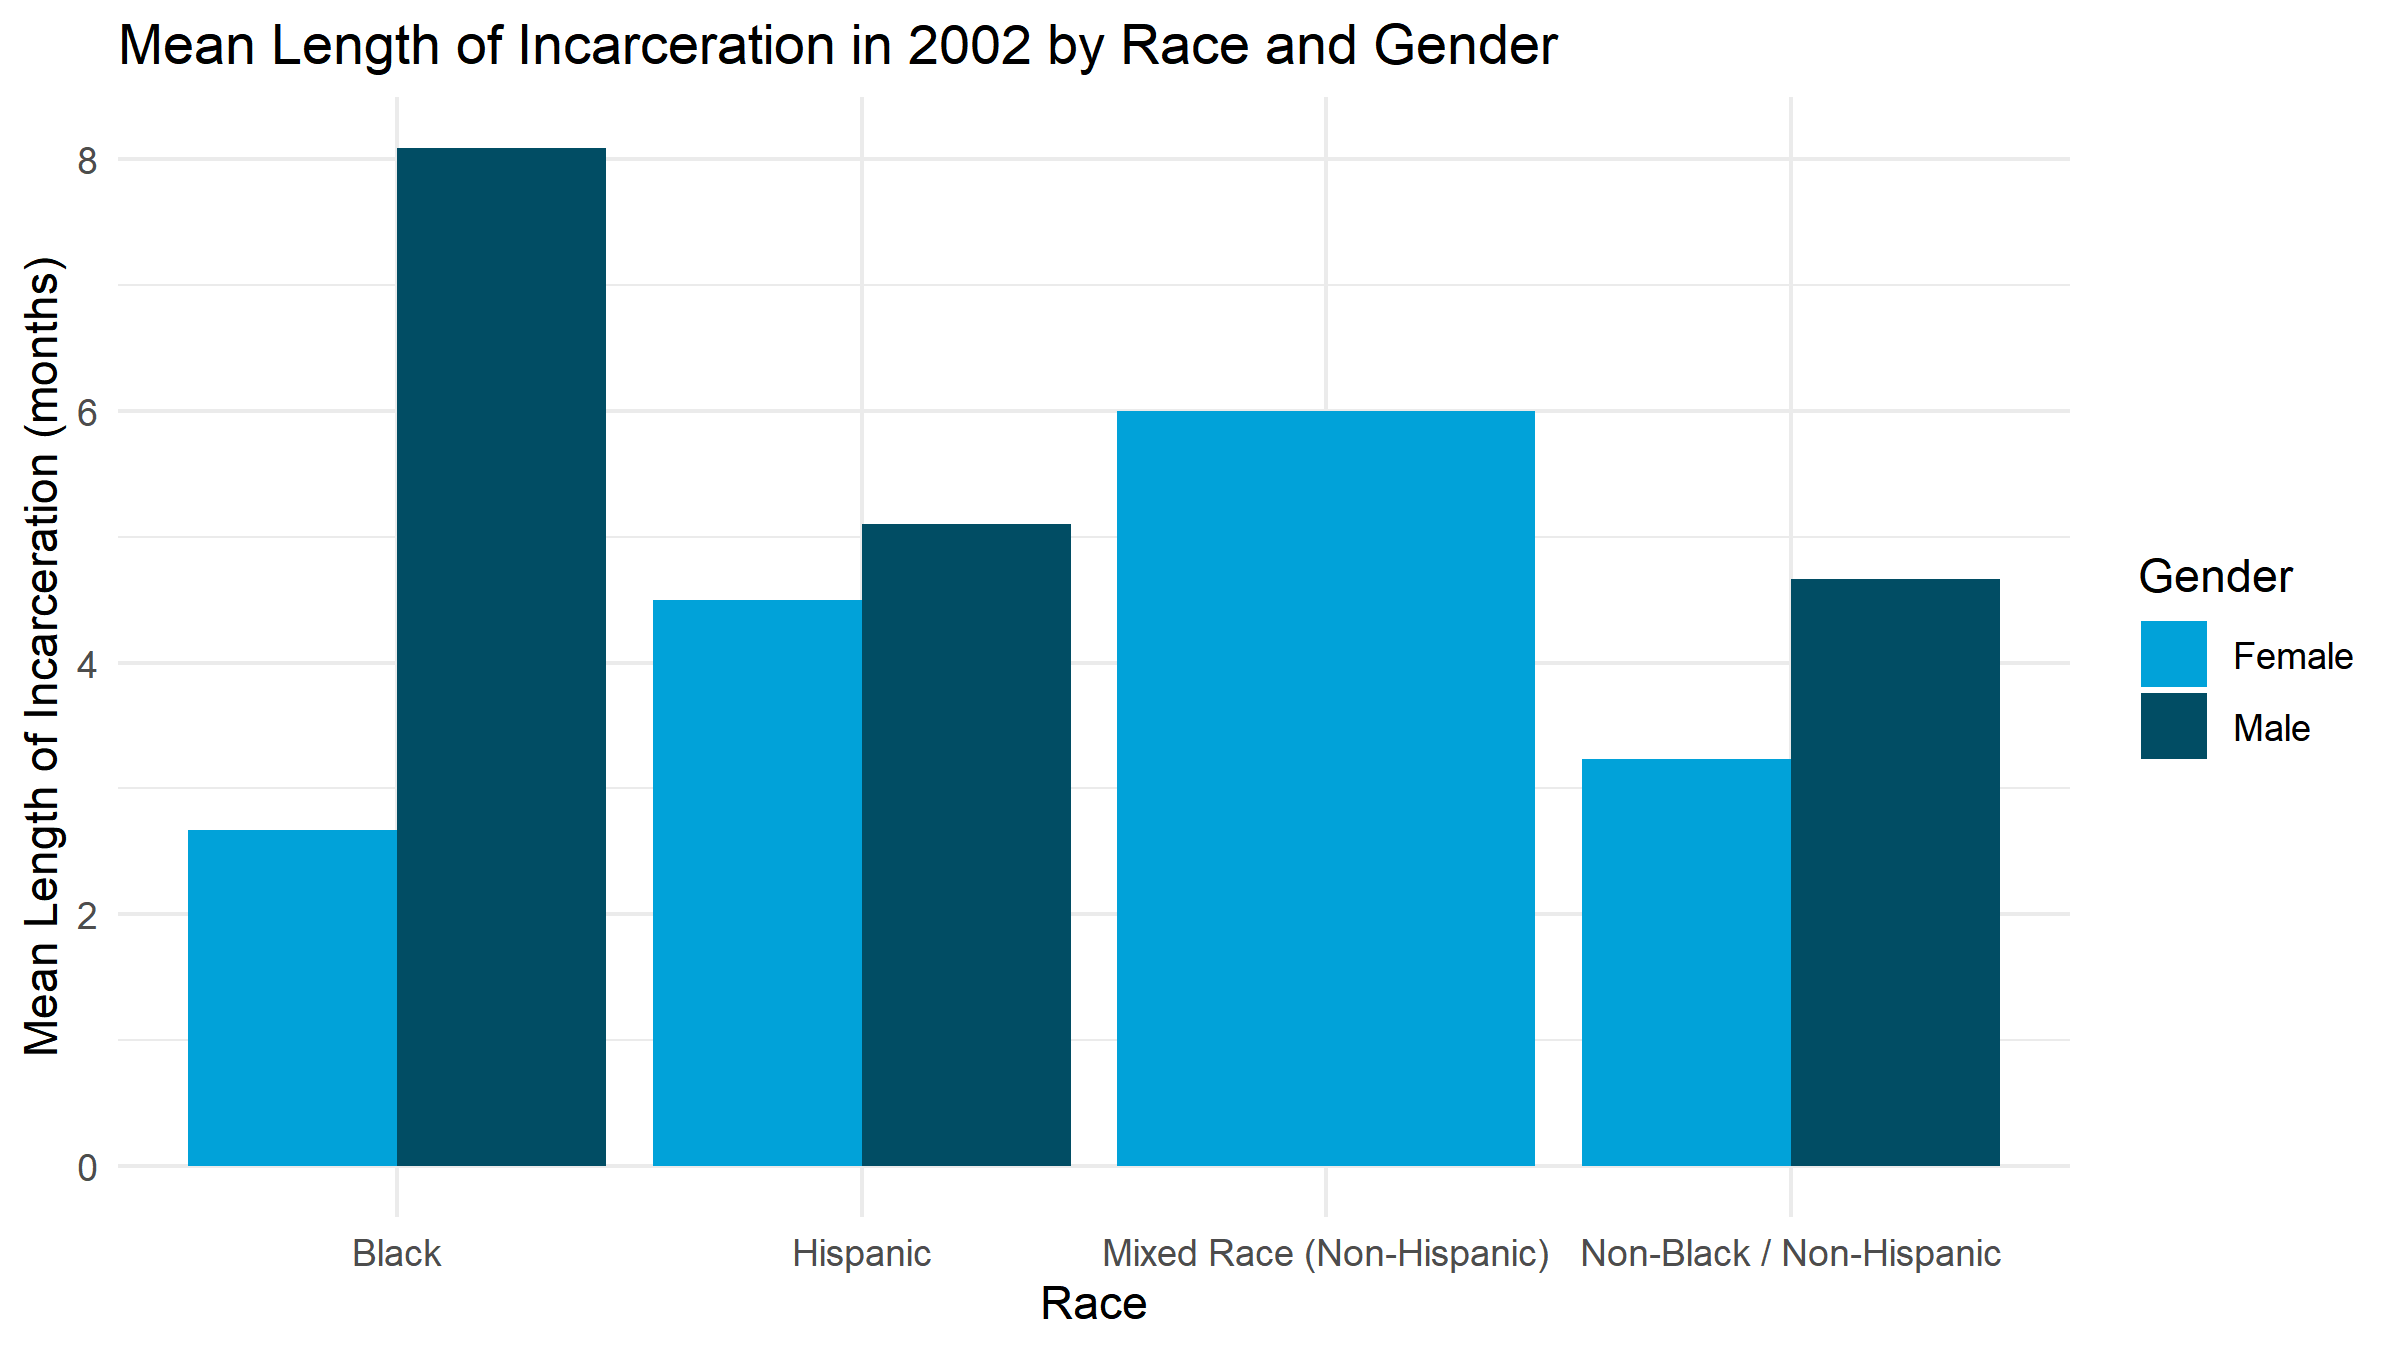
\includegraphics[width=.85\textwidth]{incar_length_by_racegender.png}
    \end{center}
    \caption{Incarcerated in 2002 by Race and Gender}
    \label{fig:graph}
\end{figure}
\begin{table}[H]

\caption{\label{tab:tab:summarystats}Mean length of incarceration in 2002 by Race and Gender}
\centering
\begin{tabular}[t]{lrrrr}
\toprule
Gender & Black & Hispanic & Mixed Race Non Hispanic & Non Black Non Hispanic\\
\midrule
\cellcolor{gray!6}{Female} & \cellcolor{gray!6}{2.666667} & \cellcolor{gray!6}{4.500000} & \cellcolor{gray!6}{6} & \cellcolor{gray!6}{3.230769}\\
Male & 8.090909 & 5.103448 & NA & 4.666667\\
\bottomrule
\end{tabular}
\end{table}



\newpage
\section{Incarceration Status Regression Analysis}


% Table created by stargazer v.5.2.2 by Marek Hlavac, Harvard University. E-mail: hlavac at fas.harvard.edu
% Date and time: Fri, Feb 18, 2022 - 11:13:32 PM
\begin{table}[!htbp] \centering 
  \caption{Regression Output. Omitted category is Black Females.} 
  \label{tab:regression} 
\begin{tabular}{@{\extracolsep{5pt}}lc} 
\\[-1.8ex]\hline 
\hline \\[-1.8ex] 
 & \multicolumn{1}{c}{\textit{Dependent variable:}} \\ 
\cline{2-2} 
\\[-1.8ex] & Length of incarceration in 2002 \\ 
\hline \\[-1.8ex] 
 Hispanic & $-$2.306 \\ 
  &  \\ 
  & \\ 
 Mixed Race (Non-Hispanic) & 0.857 \\ 
  &  \\ 
  & \\ 
 Non-Black / Non-Hispanic & $-$2.859 \\ 
  &  \\ 
  & \\ 
 Male & 2.610 \\ 
  &  \\ 
  & \\ 
 Constant & 5.143 \\ 
  &  \\ 
  & \\ 
\hline \\[-1.8ex] 
Observations & 178 \\ 
R$^{2}$ & 0.161 \\ 
Adjusted R$^{2}$ & 0.142 \\ 
Residual Std. Error & 3.946 (df = 173) \\ 
F Statistic & 8.302$^{***}$ (df = 4; 173) \\ 
\hline 
\hline \\[-1.8ex] 
\textit{Note:}  & \multicolumn{1}{r}{$^{*}$p$<$0.1; $^{**}$p$<$0.05; $^{***}$p$<$0.01} \\ 
\end{tabular} 
\end{table} 



\end{document}
